\documentclass[a4paper,12pt]{article}
\usepackage{a4wide}
\usepackage{tikz}
\usetikzlibrary{calc}

\begin{document}
\pagestyle{empty}
\setlength{\parindent}{0em} 
\section*{Arithmetic}

Your task is to program the behavior of an entity called "arithmetic". This entity is declared in the attached file "arithmetic.vhdl" and has the following properties:
\begin{itemize}
\item Inputs:  I1, I2 with type std\_logic\_vector
\item Outputs: O with type std\_logic\_vector , V with type std\_logic, C with type std\_logic, VALID with type std\_logic
\end{itemize}
\begin{center}
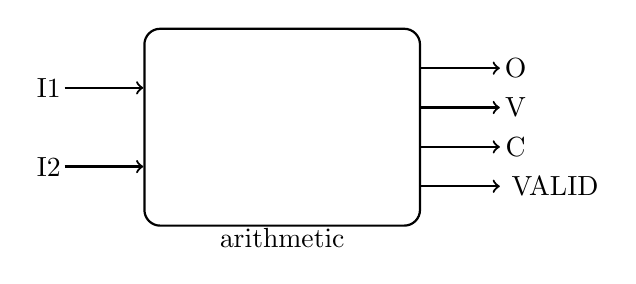
\begin{tikzpicture}
\draw node [draw,rectangle, minimum height=25mm, minimum width=35mm,rounded corners=2mm,thick](entity){};
\draw[->,thick] ($ (entity.west)-(10mm,5mm)$) -- ($ (entity.west) - (0mm,5mm)$);
\draw node at ($ (entity.west)-(12mm,5mm)$){I2};
\draw[->,thick] ($ (entity.west)-(10mm,-5mm)$) -- ($ (entity.west) - (0mm,-5mm)$);
\draw node at ($ (entity.west)-(12mm,-5mm)$){I1};

\draw[->,thick] ($ (entity.east) + (0mm,7.5mm)$) -- ($ (entity.east) + (10mm,7.5mm)$);
\draw node at ($ (entity.east) + (12mm,7.5mm)$){O};
\draw[->,thick] ($ (entity.east) + (0mm,2.5mm)$) -- ($ (entity.east) + (10mm,2.5mm)$);
\draw node at ($ (entity.east) + (12mm,2.5mm)$){V};
\draw[->,thick] ($ (entity.east) + (0mm,-2.5mm)$) -- ($ (entity.east) + (10mm,-2.5mm)$);
\draw node at ($ (entity.east) + (12mm,-2.5mm)$){C};
\draw[->,thick] ($ (entity.east) + (0mm,-7.5mm)$) -- ($ (entity.east) + (10mm,-7.5mm)$);
\draw node at ($ (entity.east) + (17mm,-7.5mm)$){VALID};


\draw node at ($ (entity) - (0,14mm)$){arithmetic};

\end{tikzpicture}
\end{center}

Do not change the file "arithmetic.vhdl".
\\

The entity shall implement the following arithmetic functionality:
\begin{itemize}
\item %%OPERATION_NAME I1 %%OPERATION_SIGN I2
\item Input operand 1 (I1): %%I1_WIDTH bit, %%OPERAND_STYLE
\item Input operand 2 (I2): %%I2_WIDTH bit, %%OPERAND_STYLE
\item Output (O): %%O_WIDTH bit, %%OPERAND_STYLE
\item Overflow (V) and Carry flag (C) set accordingly 
\item Valid flag (VALID): indicates if the computed solution is valid or not 
\end{itemize}
This behavior has to be programmed in the attached file "arithmetic\_beh.vhdl". 

\rule{16cm}{0.4pt}\par
 \subsection*{Review: Carry and Overflow Flag}
The carry flag indicates when an arithmetic carry or borrow has been generated out of the most significant ALU bit position. \\

The overflow flag indicates when an arithmetic overflow has occurred in an operation, indicating that a signed result would not fit in the number of bits used for the operation (the ALU width).\\


\textit{Source: }Wikipedia
\\
\rule{16cm}{0.4pt}

\vspace{0.3cm}

Tip: Use the ieee.numeric\_std package to implement the arithmetic operation.
\\

To turn in your solution write an email to %%SUBMISSIONEMAIL with Subject "Result Task %%TASKNR" and attach your file "arithmetic\_beh.vhdl".

\vspace{0.7cm}
Good Luck and May the Force be with you.

\end{document}